multi-scale lorem ipsum dolor sit amet

\section{Abstract}

Data sets of immense size are regularly generated on large scale
computing resources.  EVen among more traditional methods for
acquisition of volume data, such as MRI and CT scanners, data that is
too large to be effectively visualized on standard workstations is now
commonplace.

One solution to this problem is to employ a `visualization cluster,' a
small- to medium- scale cluster dedicated to performing visualization
and analysis of massive data sets generated on larger scale
supercomputers. These clusters are designed to fit a different
need than traditional supercomputers, and therefore their design
mandates different hardware choices, such as increased memory, and
more recently, graphics processing units (GPUs).  While there has
been much previous work on distributed memory visualization as well
as GPU visualization, there is a relative dearth of algorithms
that effectively use GPUs at a large scale in a distributed memory
environment.  In this work, we study a common visualization technique
in a GPU-accelerated, distributed memory setting, and present
performance charactersitcs when scaling to extremely large data sets.

\section{Introduction}

Visualization and analysis algorithms, volume rendering in particular,
require extensive compute power relative to data set size.  One
possible solution is to use the large scale supercomputer that
generated the data, which clearly has the requisite compute power.
However it can be difficuilt to reserve and obtain the compute
resources required for viewing large data sets.  An alternative
approach, one explored in this work, is to use a smaller scale
cluster equipped with GPUs.  Such a cluster can provide the needed
computational power at a fraction of the cost---provided the GPUs
can be effectively utilized.  As a result, a semi-recent trend has
emerged to procure GPU-accelerated visualization clusters dedicated
to postprocessing the data generated by high-end supercomputers;
examples include ORNL's Lens, Argonne's Eureka, TACC's Longhorn, SCI's
Tesla-based cluster, and LLNL's Gauss.

Despite this trend, there have been relatively few efforts studying distributed
memory, GPU-accelerated visualization algorithms that can effectively utiliaze
the resources available on these clusters.  In this work, we report parallel
volume rendering performance characteristics on large data sets for a typ[ical
machine of this type.

Our system is divided into three stages:

\begin{enumerate}

  \item \emph{An intelligent pre-partitioning} that is designed to make
  combining results from different nodes easy.

  \item \emph{A GPU volume renderer} to perform per-frame volume
  rendering at interactive rates.

  \item \emph{MPI-based compositing} using a sort-last compositing framework.

\end{enumerate}

M\"uller et al. presented a system similar to our own that was limited
to smaller data sets~\cite{Needed}.  We have extended the ideas in that
system to allow for larger data sets, by removing the restriction that
a data set must fit in the combined texture memory of the GPU cluster
and adding the ability to mix in CPU-based renderers, enabling us to
analyze the parallel performance on extremely large data sets.  The
primary contribution of this component of our work is an increased
understanding of the performance characteristics of a distributed
memory GPU-accelerated volume rendering algorithm at a scale (256 GPUs)
much larger than previously published.  Further, the results presented
here (data sets up to $8192^3$ voxels) represent some of the largest
parallel volume renderings attempted thus far.

Our system and benchmarks allow us to explore issues such as:

\begin{itemize}

  \item the balance between rendering and compositing: a well-studied
  issue with CPU-based rendering, but currently with unclear
  performance tradeoffs for rendering on GPU clusters;

  \item the overhead of transferring data to and from a GPU;

  \item the importance of process-level load balancing; and

  \item the viability of GPU clusters for rendering very large data.

\end{itemize}

This chapter is organized as follows.  In Section~\ref{sec:previous},
we overview previous work in parallel compositing and GPU volume
rendering.  In Section~\ref{sec:arch}, we outline our system in detail.
Section~\ref{sec:eval} discusses our benchmarks and presents their
results. Finally, in Section~\ref{sec:conclusions} we draw conclusions
based on our findings.

\begin{figure}
  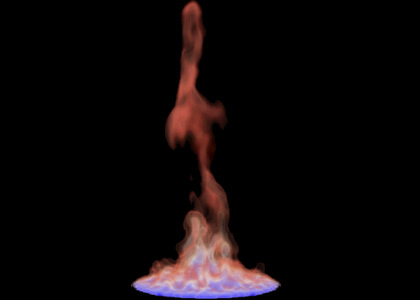
\includegraphics[width=\linewidth]{images/multiscale/teaser}
  \caption{Output of our volume rendering system with a data set
  representing a burning helium flame.}
  \label{fig:sample}
\end{figure}

\section{Previous work}
\label{sec:previous}

Volume rendering in a serial context has been studied for many years.
The
performance of the basic algorithm~\cite{Needed} was improved
significantly by incorporating empty space leaping and early ray
termination~\cite{Levoy:EarlyTermination}.  Max provided one of the
earliest formal presentations of the complete volume rendering equation
in~\cite{Needed}.  Despite significant algorithmic advances from
research such as~\cite{Levoy:EarlyTermination}, the largest increase in
performance for desktop volume renderers has come from taking advantage
of the 3D texture capabilities~\cite{Needed, Needed, Needed} and
programmable shaders~\cite{Krueger:2003:ATGV} available on modern
graphics hardware.

Extensive research has been done on parallel rendering and parallel
volume rendering.  Much of this work has focused on achieving
acceptable compositing times on large systems.  Molnar et al. conveyed
the theoretical underpinnings of rendering
performance~\cite{Molnar:199?:???}.  Earlier systems for parallel
volume rendering relied on direct send~\cite{Hsu:1993:???,
Ma:1993:???}, which divides the volume up into at least as many
chunks as there are processors, sending ray segments (fragments) to a
responsible tile node for compositing via the Porter and Duff
\emph{over} operator~\cite{PorterDuff:1984:Compositing}.  These
algorithms are simple to implement and integrate into existing systems,
but have sporadic compositing behavior and the potential to exchange a
large a number of fragments, straining the network layers when scaling
to large numbers of processors.  Tree-based compositing algorithms
feature more regular communication patterns, but impose an additional
latency that may not be required, depending on the particular frame
and data decomposition.  Binary swap and derivative algorithms are a
special case of tree-based algorithms that feature
equitable distribution of the compositing workload~\cite{Ma:1994:???}.
Despite advancements in compositing algorithms, network traffic remains
unevenly distributed in time, and thus high-performance networking
remains a necessity for subsecond rendering times on large numbers of
processors.

In the area of distributed memory parallel volume rendering of very
large data sets, the algorithm described by Ma et al
in~\cite{Ma:1993:???} has been taken to extreme scale in several
followuip publications.  In~\cite{Childs:2006:???}, data set sizes of
up to $3000^3$ are studied using hundreds of cores.  In this regime,
the time spent ray casting far exceeds the composite time.
In~\cite{PYRM:2008:???, PYR:2009:???}, the data set sizes range up to
$4480^3$, while core counts of tens of thousands are studied.
In~\cite{HBC:2010:???}, the benefits of hybrid parallelism are explored
at concurrency ranges going above two hundred thousand cores.  For both
of these studies, when going to extreme concurrency compositing time
becomes large and dominates ray-casting time.  This suggests that a
sweet spot may exist with GPU-accelerated distributed memory volume
rendering.  By using hardware acceleration, the long ray
casting times encountered in~\cite{Childs:2006:???} can be overcome.
Simultaneously, the emerging trend of composite-bound rendering
observed in~\cite{PYR:2009:???} and~\cite{HBC:2010:???} will be
mitigated by the ability to use many fewer nodes to command the same
compute power.

Numerous systems have been developed to enable parallel rendering in
existing software.  Among the most well-known is
Chromium~\cite{HHN:2002:???}, a rendering system that can transparently
parallelize OpenGL-based applications.  The Equalizer framework boasts
multiple compositing strategies, including an improved direct
send~\cite{EP:2007:???}.  The IceT library provides parallel rendering
with a variety of sort-last compositing strategies~\cite{MWP:2001:???}.

There has been less previous work studying volume rendering on
multiple GPUs.  Strengert et al. developed a system that used wavelet
compression and adaptively decompressed the data on small GPU
clusters~\cite{SMW:2004:???}.  Marchesin et al. compared a volume that
ran on two different two-GPU configurations: two GPUs on one system,
and one GPU on two networked systems~\cite{Marchesin:2008:???}.  The
use of just one or two systems, coupled with an in-core renderer,
artificially constrained the data set size.  M\"uller et al. developed
a distributed memory volume renderer that ran on
GPUs~\cite{Mueller:2006:???}; their system differs from ours in a few
key ways.  First, we use an out-of-core renderer and therefore can
exceed the available texture memory of the GPU by also utilizing CPU
memoryor disk.  To further reduce memory costs, we compute gradients
dynamically in the GLSL shader~\cite{KW:2003:???}, obviating the need
to upload a separate gradient texture.  This also has the benefit of
avoiding a pre-processing step, which is normally software-based in
existing general-purpose visualization applications (including the one
we chose to implement our system within) and can be time consuming for
large data sets.  Further differentiating our system and in line with
recent trends in visualization cluster architectures, we enable the use
of multiple GPUs per node.  M\"uller et al. used a direct send
compositing strategy~\cite{Hsu:1993:???, MPHK:1993:???}, whereas we use
a tree-based compositing method~\cite{MWP:2001:???}.  Finally, and
most importantly, we report performance results for substantially more
GPUs and much larger data sets, detailing the scalability of GPU-based
visualization clusters.  We therefore believe our work is the first
to evaluate the usability of distributed memory GPU clusters for this
scale of data.

\section{Architecture}
\label{sec:arch}

We implemented our remote rendering system inside of
VisIt~\cite{Childs:???:???}, which is capable of rendering data in
parallel on remote machines.  The system is comprised of a lightweight
`viewer' client application, connected over TCP to a server that
employs GPU cluster nodes.  All rendering is performed on the cluster,
composited via MPI, and images (optionally compressed via zlib) are
sent back to the viewer for display.  Example output from our system is
in Figure~\ref{fig:sample}.

Although VisIt provided a good starting point for our work, we needed
to make significant changes in order to implement our system.  In this
section, we highlight the main features of our system, taking special
care to note where we have deviated from existing VisIt functionality.

\subsection{Additions to VisIt}

\subsubsection{Multi-GPU access}

At the outset, VisIt's parallel server supported only a single GPU per
node.  We have revamped the manner in which VisIt accesses GPUs to
allow the system to take advantage of multi-GPU nodes.  When utilizing
GPU-based rendering, each GPU is matched to a CPU core that feeds
data to that GPU.  Additionally, when the number of CPU cores exceeds
the number of available GPUs, we allow for the use of software-based
renderers on the extra CPUs.  This code has been contributed to the
VisIt project.

\subsubsection{Partitioning}

VisIt contained a number of load decomposition stratgies prior to our
work.  However, we found these stratgies to be insufficient for a
variety of reasons:

\begin{enumerate}

  \item \textbf{Brick-based} Equalizing the distribution of work in
  VisIt was entirely based on \emph{bricks}, or pieces of the larger
  data set.  Our balancing algorithms use the time taken to render the
  previous frame to determine the weighted distribution of loads.

  \item \textbf{Master-slave} Dynamic balance algorithms in VisIt are
  based on a \emph{master} node that tells slaves to process a brick,
  waits for the slaves' completion, and then sends them a new brick to
  process.  We implemented a flat hierarchy, as seems to be more common
  in recent literature~\cite{MMD06, MSE06}.

  \item \textbf{Compositing} \emph{Most importantly}, for our
  object-based decomposition to work correctly, we needed a defined
  ordering to perform correct compositing.  The load balancing and
  compositing subsystems in VisIt were independent prior to our work.

\end{enumerate}

Our system relies on a \emph{k}d-tree for distributing and balancing
the data.  The spatial partitioning is done once initially and can
be adaptively refined by the rendering times from previous frames.
The initial tree only considers the number of bricks in the available
data set and attempts to distributed them evenly among processes, to
the extent that is possible.  When using static load balancing, this
decomposition is invariant for the life of the parallel job.
Figure~\ref{fig:decomposition} depicts a possible configuration
determined by the
partitioner, and shows the corresponding \emph{k}d-tree.

\begin{figure*}
  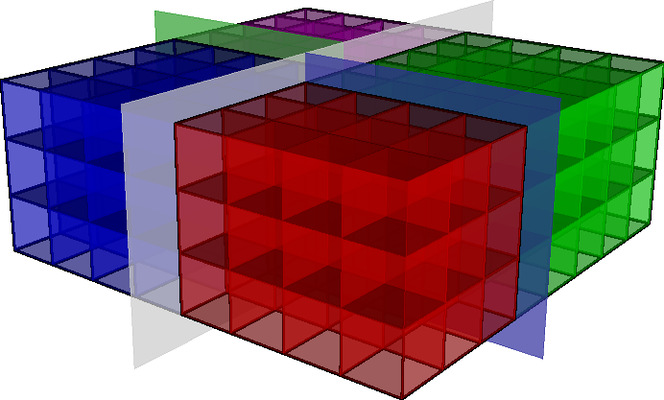
\includegraphics[width=0.49\linewidth]{images/multiscale/bricks.jpg}
  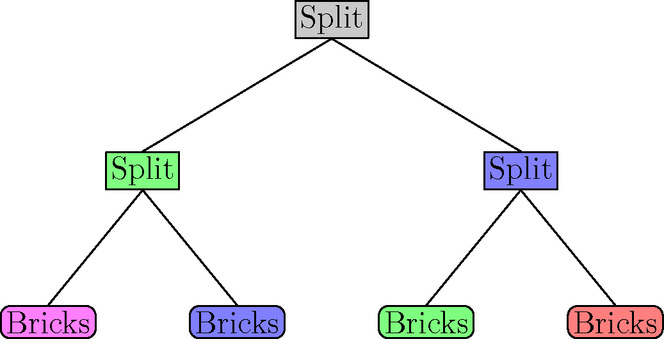
\includegraphics[width=0.49\linewidth]{images/multiscale/tree.jpg}
  \caption{Decomposition and corresponding kd-tree for an 8x8x3 grid
  of bricks divided among 4 processors.  Adjacent bricks are kept
  together for efficient rendering and compositing.  A composite order
  is derived dynamically from the camera location in relation to the
  splitting planes.  Note that the number of leaves in the tree is
  equal to the number of processes in the parallel rendering job.}
  \label{fig:decomposition}
\end{figure*}

When the dynamic load balancer is enabled, we use the last rendering
time on each process to determine the next configuration.  In our
initial implementation, the metric we utilized was the total pipeline
execution time to complete a frame.  This included the time to read
data from the disk, as well as the compositing time, among other
inputs.  However, we found that I/O would dwarf the actual rendering
time.  Further, compositing time is not dependent on the distribution
of bricks.  This therefore proved to be a poor metric.  Switching the
balancer to use the total render time for all bricks on that process
gave significantly better results.

In order to compare different implementations, we implemented multiple
load balancing algorithms, notably those described in Marchesin et al.
and M\"uller et al.'s work~\cite{MMD06, MSE06}.  In both cases, leaf
nodes represent processes, and each process has some number of bricks
assigned to it.  In the Marchesin-based approach, we start at the
parents of the leaf nodes and work our way up the tree, searching for
imbalance among siblings.  If two siblings are found to be imbalanced,
a single layer of bricks is moved along the splitting plane.  This
process continues up the root of the tree, at which time the virtual
results are committed and the new tree dictates the resulting data
distribution.  In the M\"uller-based approach, we begin with the root
node and use a pre-order traversal to find imbalance among siblings.
Once imbalance is found, the process stops for the current frame.
Instead of blindly shifting a layer of bricks between the siblings,
the method derives the average rendering cost associated with a layer
of bricks along the split plane, and shifts this layer if the new
configuration is projected to improve rendering time.

In addition to achieving a relatively even balance among the data, the
\emph{k}d-tree is used in the final stages to derive a valid sort-last
compositing order.

\section{Evaluation}
\label{sec:eval}

\section{Conclusions}
\label{sec:conclusions}
